\section{Evaluation}

We use this web layout algorithm
  to compare Spineless Traversal
  against the Double Dirty Bit algorithm
  on \NumWebsites real-world websites.

\subsection{Benchmarks}

To evaluate web layout for these websites,
  we modified the Ladybird web browser
  to dump the layout tree at every rendered frame;
  we then use a separate program to ``diff'' successive frames,
  outputting a list of insertions, deletions,
  and attribute/property changes.
A benchmark program then reads the diff
  and performs each modification in the list,
  then invokes the incremental layout entry point.
Both invalidation and recomputation time
  are measured using the \texttt{rdtsc} instruction,
  allowing a granular comparison of both
  Spineless Traversal and Double Dirty Bit.
In total, the \NumWebsites websites generate traces
  with \NumFrames frames in total.
Each frame leads to a single incremental layout call,
  so our experiment has \NumFrames individual data points.
Note that this large number of frames,
  covering gigabytes of layout tree data,
  nonetheless represents only a few minutes of web browsing activity.
All experiments are run on a machine with
  an Intel i7-8700K CPU (8th generation)
  clocked at the standard 3.70\,GHz
  with 64\,KB L1 cache, 256\,KB L2 cache (both per core),
  and 12\,MB L3 cache, plus
  32\,GB of DDR4 memory across 4 DIMMs,
  each configured to 3000 MT/s.

The \NumWebsites real-world websites include
  Amazon, Wikipedia, Github, Google,
  as well as a number of other popular websites
  drawn from the Alexa ranking of top websites
  and focusing on large web pages and complex web applications.
It also includes a number of personal favorites of the authors,
  including Github and Lichess.
We focus on latency-sensitive interactions
  like hovering, typing, dragging, and animations.
These interactions typically
  do not require loading data over the network
  and invalidation time is thus a big determinant of their latency.
By contrast, interactions like loading a whole web page
  or moving between portions of a website
  typically have network latency which far overshadows
  any possible invalidation latency.
Even though the interactions may seem minor,
  it is important to note that the browser is nonetheless
  performing a significant amount of work to render them.
For example, on Wikipedia, hovering over a link
  shows a ``preview'' window,
  and Wikipedia code must track and respond to mouse movements
  to hide and show the preview window at the correct time.
Moreover, there is a short, nearly-imperceptible animation
  by which the preview window slides and fades in and out of view.
Similarly, on the Lichess web page,
  our trace captures one of the authors
  stepping through a chess opening using the website's
  chess commentary tools.
The Lichess website renders the chess board using HTML elements
  and each move animates visual aids like arrows.
Text editing, an especially latency-sensitive interaction,
  was also tested.
For example, on the Google website we tested
  typing a search term letter by letter,
  with the Google website changing autocomplete suggestions
  as we typed.

\subsection{Results}

\begin{figure}
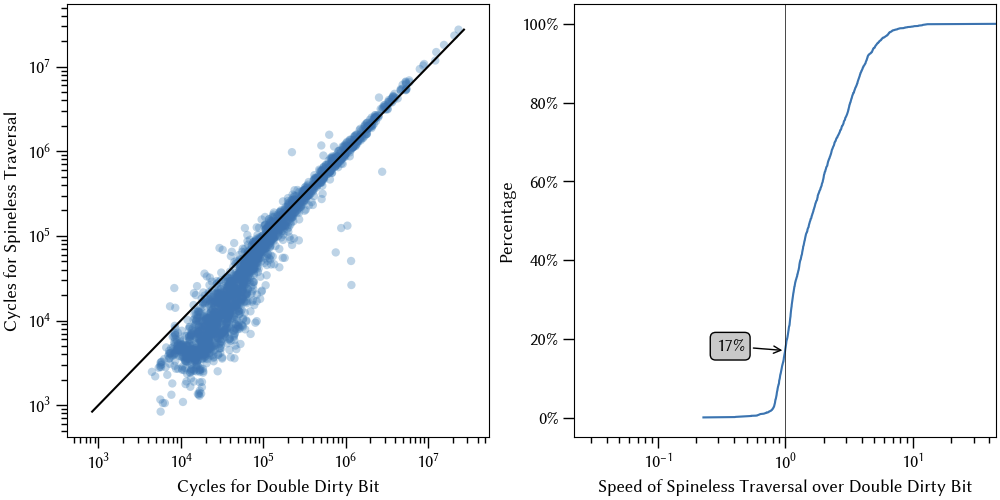
\includegraphics[scale=0.4]{DBPQ.png}
\begin{minipage}[t]{0.48\linewidth}
\caption{
The invalidation traversal time for all \NumFrames frames,
    with Double Dirty Bit time on the $x$ axis
    and Spineless Traversal time on $y$ axis.
The diagonal line shows the $x = y$ equal time line;
    points below the line are faster with Spineless Traversal
    while points above the line are faster with Double Dirty Bit.
Both axes are in log scale, meaning Spineless Traversal is often
    tens or hundreds of times faster than Double Dirty Bit.
}
\label{fig:xy}
\end{minipage}\hfill%
\begin{minipage}[t]{0.48\linewidth}
\caption{
  A CDF of the ratio between
    Double Dirty Bit time and Spineless Traversal time
    for each frame.
  The vertical line, at $10^0$,
    marks where both invalidation algorithms take equal time.
  To the left of the line,
    \PctSlower of frames are slower with Spineless Traversal.
  To the right of the line,
    \PctFaster of frames are faster with Spineless Traversal.
  The geometric mean speedup with Spineless Traversal
    is \MeanSpeedup.}
\label{fig:cdf}
\end{minipage}
\end{figure}

\iffalse
\begin{figure}
\begin{subfigure}{0.5\linewidth}
    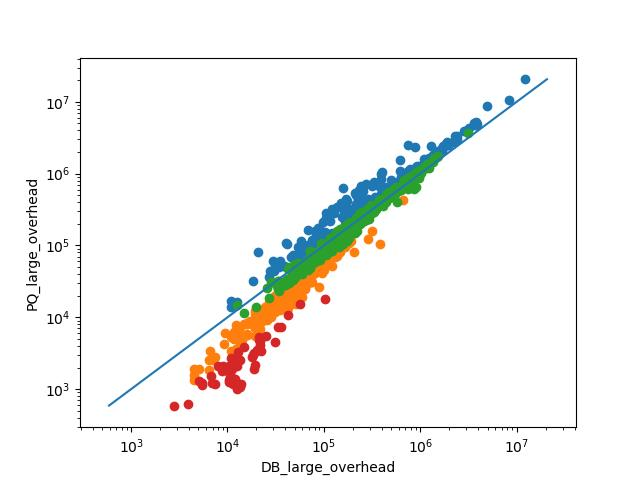
\includegraphics[width=\linewidth]{DBPQLargeOverhead.png}
\end{subfigure}\hfill%
\begin{subfigure}{0.5\linewidth}
    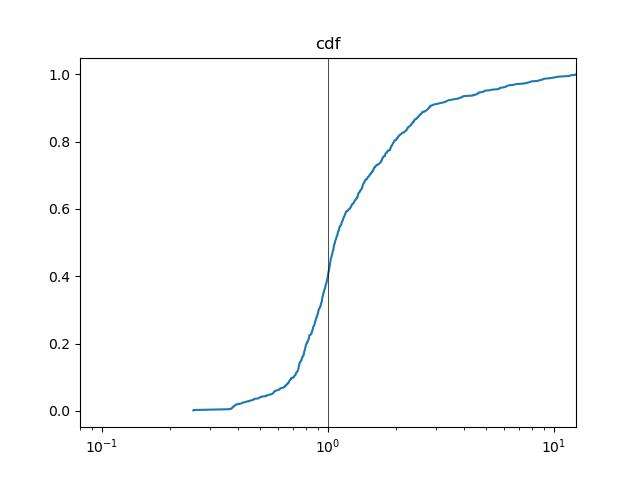
\includegraphics[width=\linewidth]{DBPQLargeCDF.png}
\end{subfigure}
\caption{
The overhead scatter plot and the speedup cdf,
  restricted to frames where more than 1\% of fields
  are recomputed. These points typically represent loading of new contents.}
\label{fig:dbpq-large}
\end{figure}
\fi

Figure~\ref{fig:xy}
  shows our results.
In Figure~\ref{fig:xy}, points below the diagonal line
  are faster with Spineless Traversal,
  while points above the diagonal line
  are faster with Double Dirty Bit.
Most points are below the line,
  often with enormous speedups: 10--$100\times$.
These points are often interactions
  where only a few deeply-nested nodes are dirtied,
  where Double Dirty Bit accesses a huge number
  of auxiliary nodes.
By contrast, while some points are above the line,
  meaning they are slower with Spineless Traversal,
  they are typically much closer to the line,
  indicating that slowdowns are not as severe
  as the speedups are beneficial.
The geometric mean is a \MeanSpeedup speedup
  from Spineless Traversal,
  with only \PctSlower of frames rendered slower.
Figure~\ref{fig:cdf} shows CDF of the speedup
  of Spineless Traversal over Double Dirty Bit.

Figures~\ref{fig:xy} and~\ref{fig:cdf} show
  only invalidation time,
  including traversal, dirty bit propagation,
  enqueuing nodes in the priority queue (for Spineless Traversal)
  and setting summary bits (for Double Dirty Bit).
We measured field computation time separately,
  and confirmed that it was nearly identical
  between Spineless Traversal and Double Dirty Bit,
  which is as expected since both algorithms will
  recompute the exact same fields in the exact same order.
In total, invalidation time was roughly one third of total runtime,
  while field computation time was roughly two thirds,
  showing that invalidation is a determinant of latency.

A more careful inspection of Figure~\ref{fig:xy} shows
  several additional features.
The slowest frames all feature slowdowns.
This is expected: the slowest frames likely represent
  the initial page load or other ``loading'' frames,
  which we necessarily capture in our traces.
While speedups are always better than slow-downs,
  these loading frames likely follow network latency,
  so invalidation time for these frames is less important.
Meanwhile, frames where fewer nodes are invalidated
  are typically those triggered in response to
  an animation or user interaction,
  where latency is most critical.
Figure~\ref{fig:dbpq-small} shows an analog of
  Figures~\ref{fig:xy} and~\ref{fig:cdf}
  but restricted to points where fewer than 1\% of fields
  are recomputed;
  the intention is that a loading frame typically changes
  large portions of the web page
  while interactions typically change much less.
On this latency-critical subset,
  which contains more than half of frames,
  the geometric mean speedup is larger,
  at \MeanSpeedupSmall,
  and a smaller fraction of frames suffer slowdowns.

\begin{figure}
    \centering
    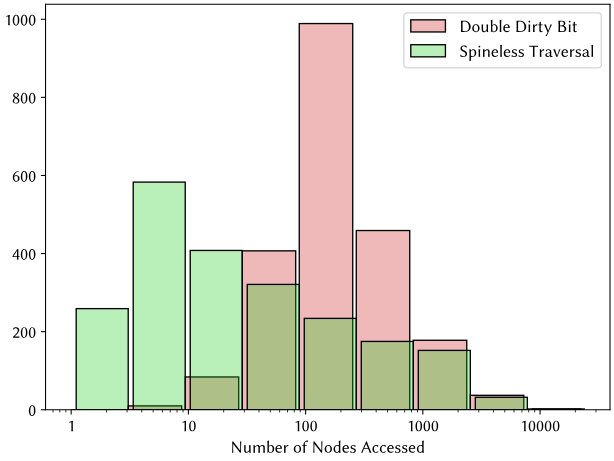
\includegraphics[width=0.5\linewidth]{DBPQHist.png}
\label{fig:nodes-accessed}
\caption{Histograms of Number of Nodes Accessed by Double Dirty Bit and Spineless Traversal. Double Dirty Bit access much more nodes compare to Spineless Traversal, so the latter cause much fewer cache misses.}
\end{figure}

Spineless Traversal is also faster on average outside this subset,
  likely because the 1\% threshold is an imprecise heuristic,
  but the dramatically larger speedup 
  in this latency-critical subset
  supports the idea that Spineless Traversal helps most
  precisely on those points where latency is most important.

\begin{figure}
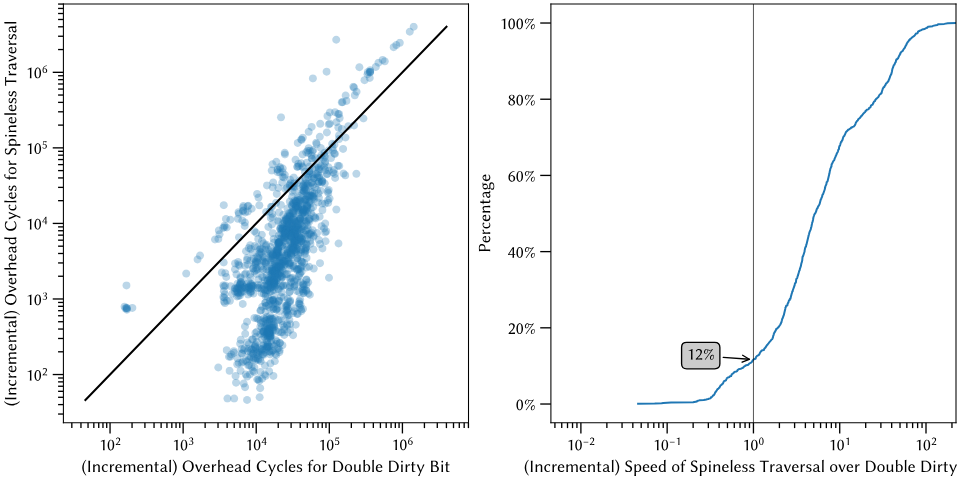
\includegraphics[scale=0.4]{DBPQSmall.png}
\begin{subfigure}{0.48\linewidth}
\end{subfigure}\hfill%
\begin{subfigure}{0.48\linewidth}
\end{subfigure}
\caption{The overhead scatter plot and the speedup CDF,
  restricted to frames where fewer than 1\% of fields
  are recomputed.
  These frames typically represent the latency-sensitive
  interactions like hovering, animations or editing.}
\label{fig:dbpq-small}
\end{figure}

\subsection{Case Study: Twitter}
To gain a deeper understanding of Spineless Traversal,
  we focus on Twitter (now X), a social media platform.
More specifically,
  we focus on the 125 incremental layouts performed
  to opened the Twitter news feed,
  load the default number of tweets,
  and scroll down repeatedly to load more tweets.
Twitter is a large web page,
  with the tree growing to 3700 DOM nodes.
This tree has a depth of 53,
  a maximum child count of 128,
  and some nodes having as many as 134 auxiliary nodes. 
Considering all the frames in aggregate,
  Twitter sees a mean speedup of $4.36\times$ 
  over the Double Dirty Bit algorithm.

Most of the 125 incremental layouts are small,
  dirtying no more then 20 nodes (Figure~\ref{fig:case-study}).
For these frames,
  incremental layout spends most of its time
  accessing auxiliary nodes.
However, the largest incremental layout
  dirties several hundred nodes.
The 125 incremental layouts are triggered
  by a variety of causes.

\begin{figure}
\begin{subfigure}{0.48\linewidth}
    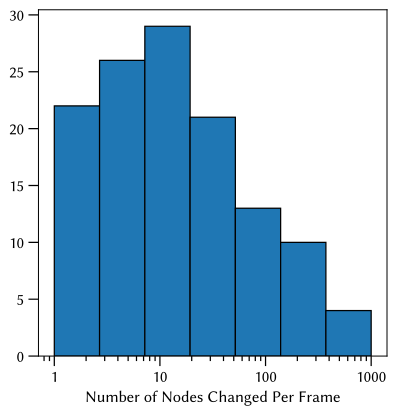
\includegraphics[scale=0.45]{CaseStudy.png}
    \caption{The numbers of nodes changed externally for each frame, for Twitter. Most frames are very incremental, with 79 frames changing no more than 20 nodes in the tree. However there are some very large changes caused by content insertion/removal, with the largest change being 787 nodes in a single frame.}
    \label{fig:case-study}
\end{subfigure}\hfill%
\begin{subfigure}{0.48\linewidth}
    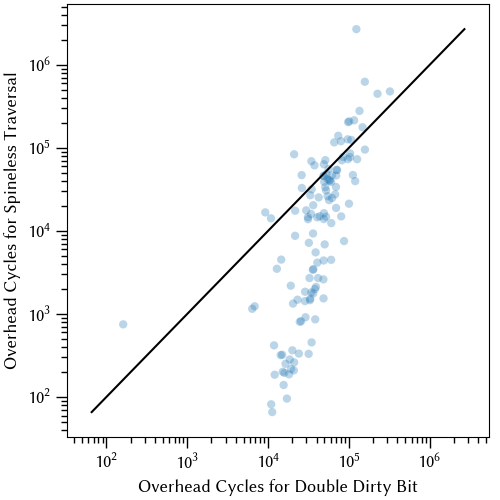
\includegraphics[scale=0.5]{CaseStudyOverhead.png}
    \caption{The overhead scatter plot of Spineless Traversal compared to Double Dirty Bit for Twitter. Most points are below the $y=x$ line, indicating a speedup. Moreover, there are many points providing large speedup of over an order of magnitude.}
\end{subfigure}
\end{figure}

\paragraph{Linked Files}
Many layouts are triggered when linked files---%
  JavaScript, CSS, images, and videos---%
  finish loading.
Loading JavaScript might add
  new \texttt{<script>} and \texttt{<style>} elements to the page,
  while loading CSS can affect the CSS properties
  of existing elements.
Loading images and videos, meanwhile,
  changes inherent width and height attributes
  (from 0 to the actual image width/height)
  used to compute a layout node's intrinsic size.
Typically only one or a few nodes are dirtied,
  but these nodes have many auxiliary nodes.
Most image and video nodes, for example
  are located deep in the layout tree,
  while \texttt{<script>} and \texttt{<style>} nodes
  are close to the root but have a huge number of siblings.
Spineless Traversal thus dramatically speeds up
  these incremental layouts,
  by up to $100\times$ in extreme cases.
 
\paragraph{Lazy Loading}
Twitter uses a lazy-loading technique
  which first loads a ``shell'' page
  and then gradually adds more and more elements to the shell
  as more content is loaded over the network.
For example, the header bar, side bar, ads, and tweets
  all load in separate frames and thus require
  separate incremental layouts.
Scrolling causes yet more content (tweets and ads) to load.
These frames, typically insert a single large subtree.
Despite the bulk insertion optimizations
  described in Section~\ref{sec:tree-insertion},
  these are still difficult for Spineless Traversal
  because it must create a large number of new OM objects
  and then rebalance the OM data structure.
Spineless Traversal is thus slower than Double Dirty Bit on these frames,
  typically by about $2\times$.
However, note that the latency in this case is partially hidden
  by the network latency of loading the content in the first place,
  so the slowdown here is likely less critical than for other frames.

\paragraph{Removal}
The Twitter application also occasionally removes
  remove parts of the page that are no longer visible to the user.
For example, offscreen content is sometimes removed;
  Spineless Traversal handles these removals
  much faster than Double Dirty Bit,
  often by $10\times$ or more,
  since Twitter is removing exactly those elements
  that do not affect what the user sees on the screen.
Twitter also sometimes removes
  individual \texttt{<script>} and \texttt{<style>} elements
  that don't affect the page;
  here Spineless Traversal's speedup
  is smaller, approximately $2\times$,
  as multiple \texttt{<script>}/\texttt{<style>} are removed at once,
  amortizing cost of accessing auxiliary nodes in Double Dirty Bit. 

Moreover, some frames mix file loading, lazy loading, and removals,
  simply due to whether these occur in the same or different frames;
  in this case the time taken for Spineless Traversal 
  basically sums over the time for each individual change,
  while Double Dirty Bit can amortize the cost
  of traversing auxiliary nodes.
As a result, these mixed frames typically see smaller speedups;
  however, these frames are still typically small
  (often many images loading at once)
  so Spineless Traversal still sees a significant speedup.
